% !TEX program = xelatex
% basic document config
\documentclass[a4paper,10pt,xetex]{article}
\usepackage[a4paper,top=45mm,right=20mm,bottom=30mm,left=25mm,head=35mm,foot=20mm]{geometry}

% language
\usepackage[german]{babel}

% variable definitions
\providecommand{\documenttitle}{Bedienungsanleitung}
\providecommand{\documentauthors}{Andreas Saurer \\ Benjamin Schneidinger \\ Josef Erben \\ Raffaele Bof \\ Nicolas Loth}
\providecommand{\documentdate}{16.05.2017}
\providecommand{\documentversion}{1.0.0}

% special commands
\newcommand*{\fullref}[1]{\hyperref[{#1}]{\nameref*{#1} (\ref*{#1})}}
\newcommand{\specialcell}[2][c]{%
  \begin{tabular}[#1]{@{}l@{}}#2\end{tabular}}

% font
% \usepackage{titling}
\usepackage[sfdefault]{roboto}
\usepackage[parfill]{parskip}
\usepackage{soul}

% table
\usepackage{array}
\usepackage{multicol}
\usepackage{longtable,tabu,booktabs}

% links
\usepackage{hyperref}
\hypersetup{
            pdftitle={\documenttitle},
            pdfauthor={\documentauthors},
            colorlinks=true,
            linkcolor=[RGB]{74,144,226},
            citecolor=[RGB]{74,144,226},
            urlcolor=[RGB]{74,144,226},
            breaklinks=true}
\urlstyle{same}  % don't use monospace font for urls

% images
\usepackage[font=small,skip=6pt]{caption}
\usepackage{float,graphicx,grffile,wrapfig}
\graphicspath{ {images/} }

\makeatletter
\def\maxwidth{\ifdim\Gin@nat@width>\linewidth\linewidth\else\Gin@nat@width\fi}
\def\maxheight{\ifdim\Gin@nat@height>\textheight\textheight\else\Gin@nat@height\fi}
\makeatother
\setkeys{Gin}{width=\maxwidth,height=\maxheight,keepaspectratio}

\makeatletter
\def\fps@figure{H}
\makeatother

% header and footer
\usepackage{lastpage}
\usepackage{fancyhdr}
\pagestyle{fancy}
\fancyhf{}
\fancyhead[L]{
\includegraphics[height=2cm]{travel-buddy_white}}
\fancyfoot[L]{\fontsize{8}{10}\selectfont\ \documenttitle}
\fancyfoot[R]{\fontsize{8}{10}\selectfont\ Seite\ \thepage\ von\ \pageref*{LastPage}}

\renewcommand{\headrulewidth}{0pt}
\renewcommand{\footrulewidth}{0pt}

% style titles
\usepackage{titlesec}
\titlespacing*{\section}{0pt}{1em}{0pt}
\titlespacing*{\subsection}{0pt}{1em}{0pt}
\titlespacing*{\subsubsection}{0pt}{1em}{0pt}

% configure title page
\title{
  
\includegraphics[width=7cm]{travel-buddy_white}\\[\bigskipamount]
  \documenttitle\\[\bigskipamount]
}

\author{\documentauthors}
\date{\parbox{\linewidth}{\centering%
  IT15TA ZH \hspace*{3cm} Gruppe 3\endgraf\bigskip
  Dokumentversion \documentversion, \documentdate\endgraf
}}


\begin{document}
\shorthandoff{"}

% title page
\maketitle\newpage

% table of contents
% {
% \hypersetup{linkcolor=black}
% \setcounter{tocdepth}{3}
% \renewcommand{\baselinestretch}{0.99}\normalsize
% \tableofcontents
% \renewcommand{\baselinestretch}{1.0}\normalsize
% }
%
% \newpage

% start content
\section{TravelBuddy - Your travel companion}
% TODO check slogan

TravelBuddy stellt dir in deiner Lieblingsstadt eine Route der wichtigsten Sehenswürdigkeiten
zusammen. Egal ob du nur ganz spontan wenige Stunden zeit hast, oder ob du eine mehrtägige
Tour planst.

Die verschiedenen Wegpunkte läufst oder fährst du in deinem Tempo - mit dem Fortbewegungsmittel
deiner Wahl - ab. An einem Wegpunkt angelangt kannst du die überwältigenden Eindrücke auf
einem Foto festhalten. TravelBuddy überprüft deinen Standort und zeigt dir danach den Weg
zum nächsten Standort auf. Am Schluss siehst du eine Übersicht über die ganze Tour und
deine erstellten Fotos.

\subparagraph{Hinweis Demoversion:}
Bitte den jeweiligen Abschnitt vor einer Aktion komplett lesen! Teilweise müssen
Anweisungen für die Demoversion vor den im Abschnitt erwähnten Aktionen ausgeführt werden.

\subsection{Tour wählen}
Wenn du TravelBuddy startest, erhälst du einen Überblick über die gängigsten Touren in
deiner Nähe (\hyperref[fig:list-activity]{Abbildung~\ref*{fig:list-activity}}).
Tippe auf eine Tour deiner Wahl um weitere Informationen und eine
Routenübersicht zu erhalten (\hyperref[fig:detail-activity]{Abbildung~\ref*{fig:detail-activity}}).

\begin{figure}
  \centering
  \begin{minipage}[b]{0.48\textwidth}
    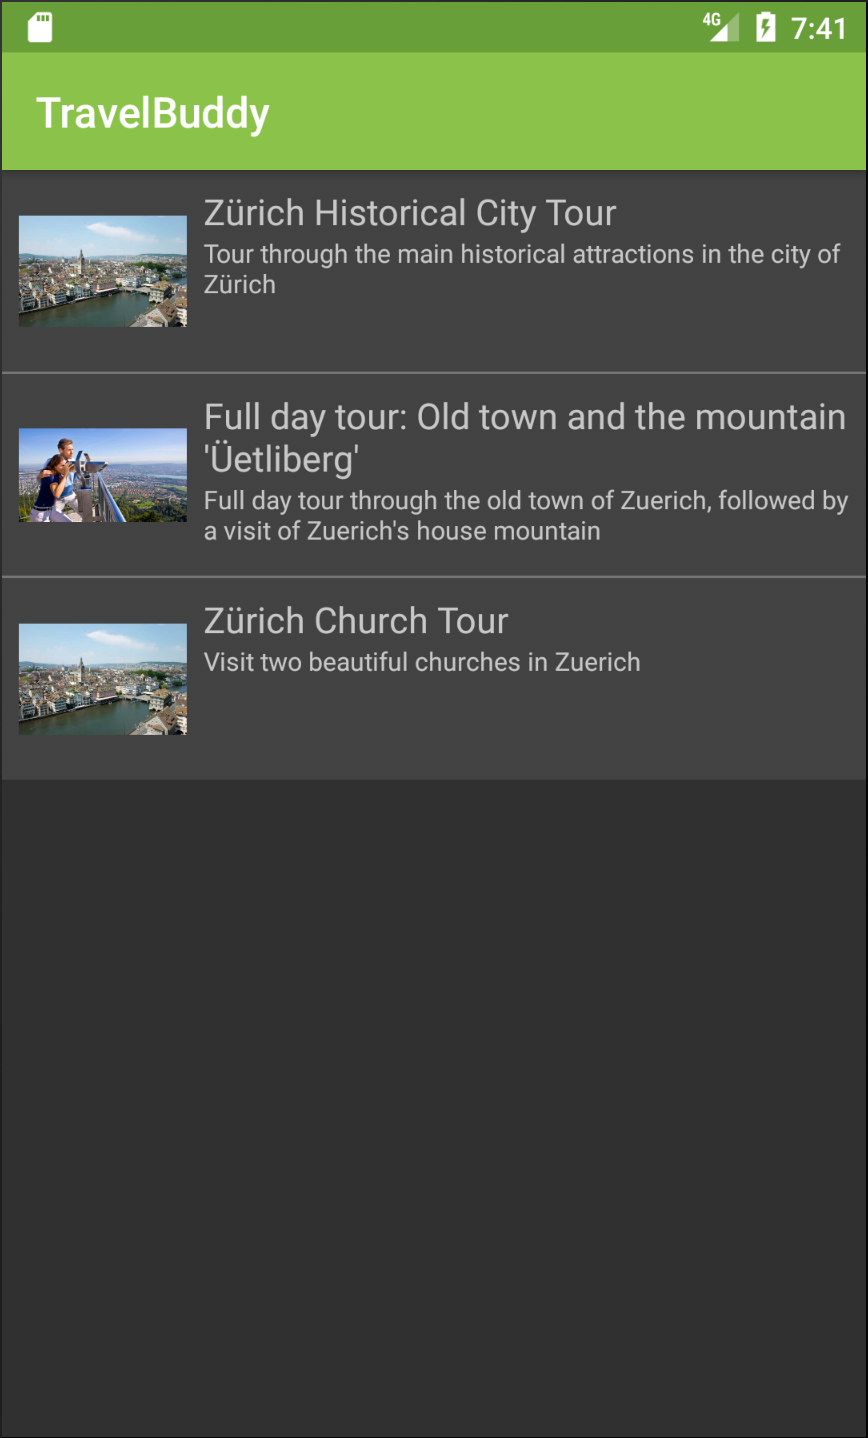
\includegraphics[width=\textwidth]{screenshots/ListActivity}
    \caption{Startbildschirm von TravelBuddy}
    \label{fig:list-activity}
  \end{minipage}
  \hfill
  \begin{minipage}[b]{0.48\textwidth}
    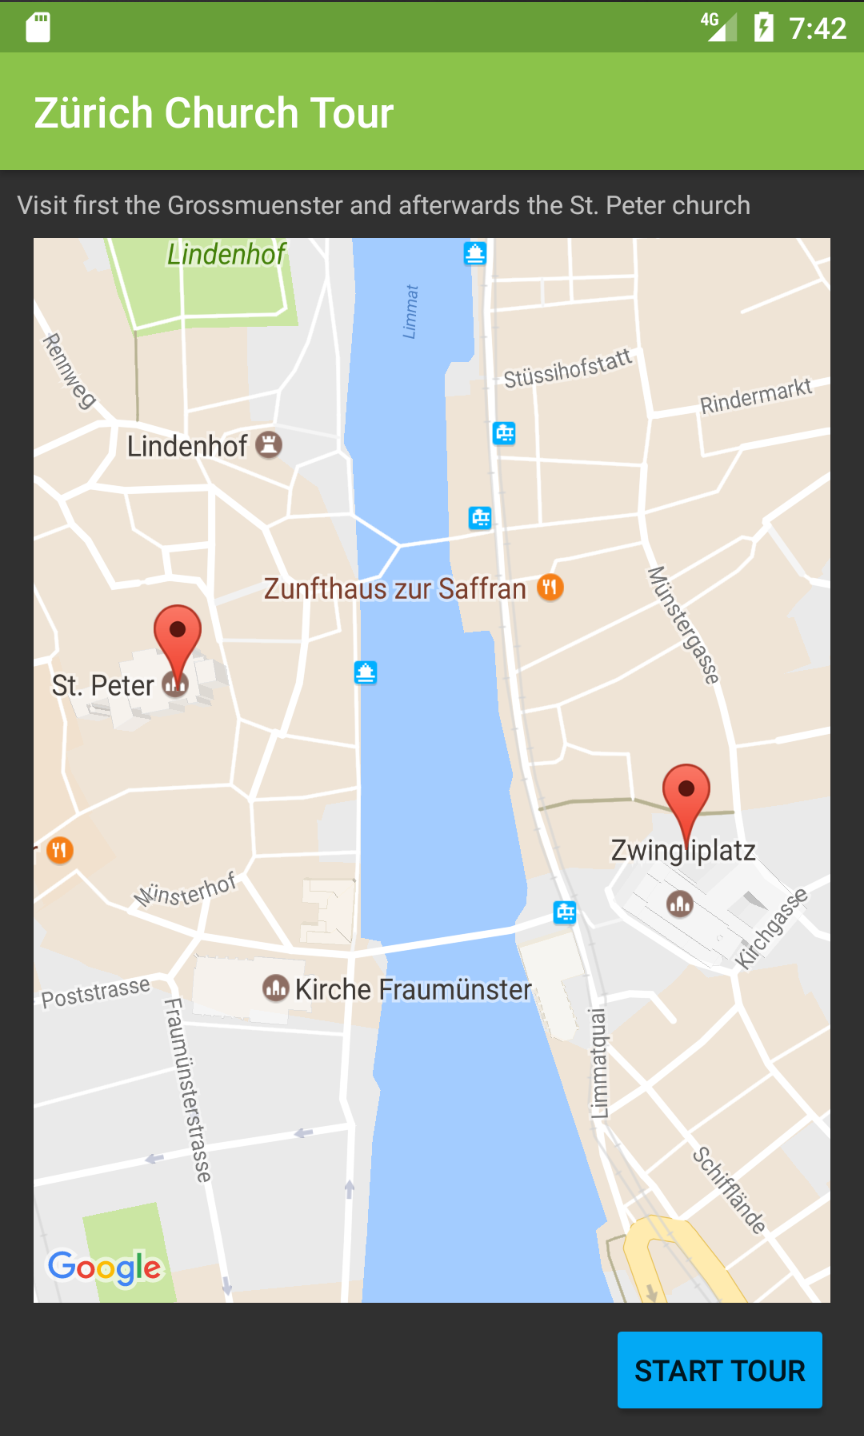
\includegraphics[width=\textwidth]{screenshots/DetailActivity}
    \caption{Detailansicht einer Tour}
    \label{fig:detail-activity}
  \end{minipage}
\end{figure}

\subparagraph{Hinweis Demoversion:}
Möglicherweise läuft das Backend (der Server, welcher die Touren zur verfügung stellt) beim
öffnen noch nicht und TravelBuddy kann somit keine Touren laden. Falls keine Touren geladen
werden, einfach die App schliessen und wieder öffnen.

Bitte die Tour ``Zürich Church Tour'' wählen, da wir hierfür Demo GPS Daten mitgeliefert haben.

\subsection{Tour starten}

Sobald du eine Tour angetippt hast, erscheint zuunterst ein Knopf ``Tour starten''
mitwelchem du die Tour startest (\hyperref[fig:detail-activity]{Abbildung~\ref*{fig:detail-activity}}).
Dir wird nun die Route zum ersten Wegpunkt angezeigt (\hyperref[fig:tour-activity]{Abbildung~\ref*{fig:tour-activity}}).
Begib dich nun auf den Weg zum ersten Punkt.

\begin{figure}
  \centering
  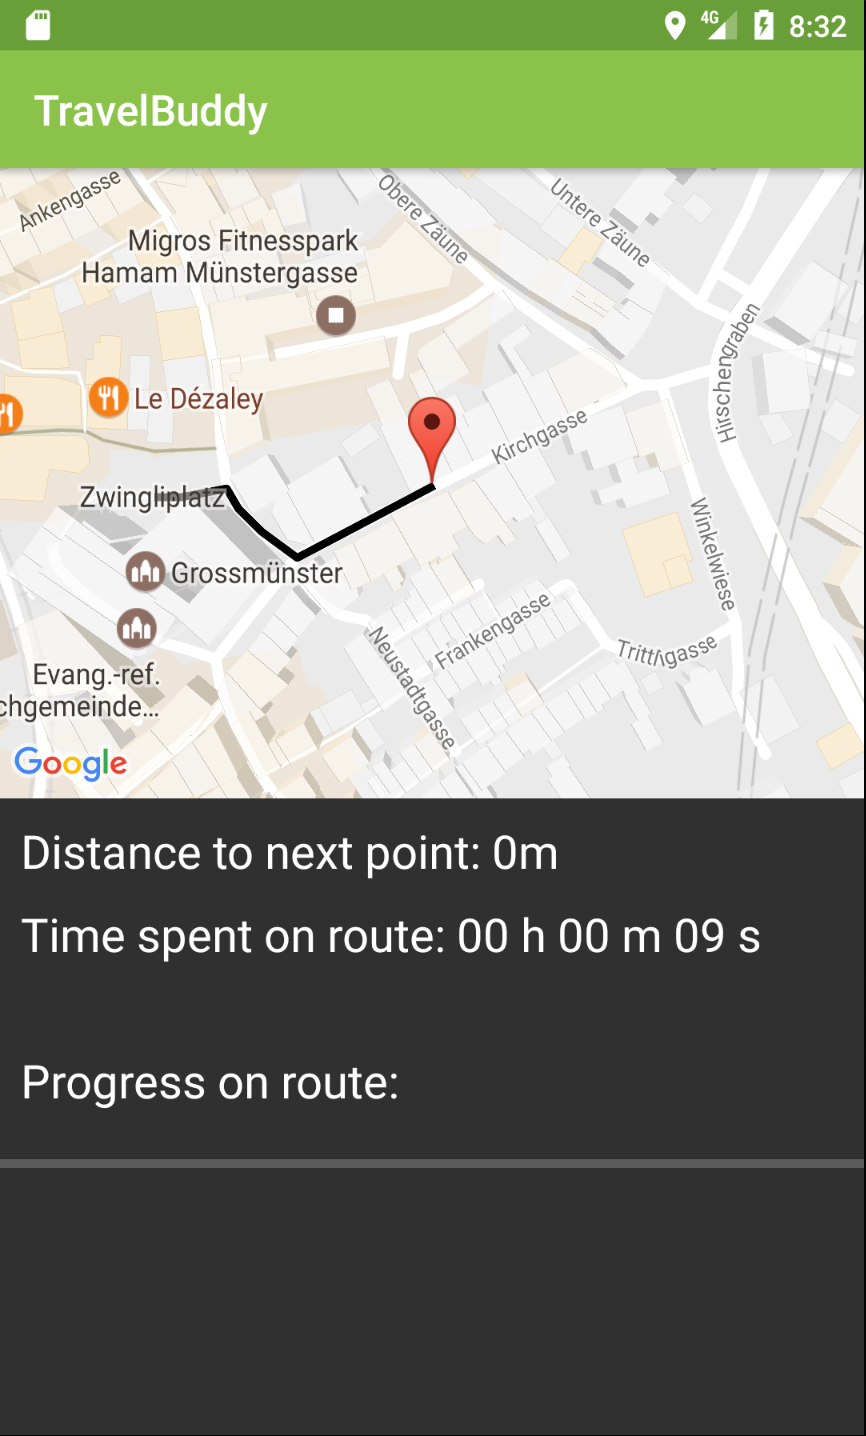
\includegraphics[width=0.48\textwidth]{screenshots/TourActivityStart}
  \caption{Route zum ersten Wegpunkt deiner Tour}
  \label{fig:tour-activity}
\end{figure}

\subparagraph{Hinweis Demoversion:}
Bevor die Tour gestartet werden kann, müssen die GPS Daten eingelesen werden. Hierzu
die drei Punkte anklicken (\hyperref[fig:android-emulator-sidebar]{Abbildung~\ref*{fig:android-emulator-sidebar}})
und im darauf erscheinenden Dialog-Fenster unten rechts auf ``Load GPX/KML'' klicken
(\hyperref[fig:android-emulator-extended-controls]{Abbildung~\ref*{fig:android-emulator-extended-controls}}, Nr. 1).
Anschliessend im Datei-Dialog die Datei ``demo\_route.gpx'' aus dem in der
Installationsanleitung angegebenen Ordner laden. Nun sollten im zuvor leeren
weissen Feld (\hyperref[fig:android-emulator-extended-controls]{Abbildung~\ref*{fig:android-emulator-extended-controls}}, Nr. 2)
diverse GPS Datenpunkte (Längen- und Breitengrade) erscheinen. Nach diesen
Schritten kann die Tour wie oben beschrieben gestartet werden.

\begin{figure}
  \centering
  \begin{minipage}[b]{0.28\textwidth}
    
\includegraphics[height=8cm]{screenshots/EmulatorSidebar}
    \caption{Sidebar des Android Emulators}
    \label{fig:android-emulator-sidebar}
  \end{minipage}
  \hfill
  \begin{minipage}[b]{0.68\textwidth}
    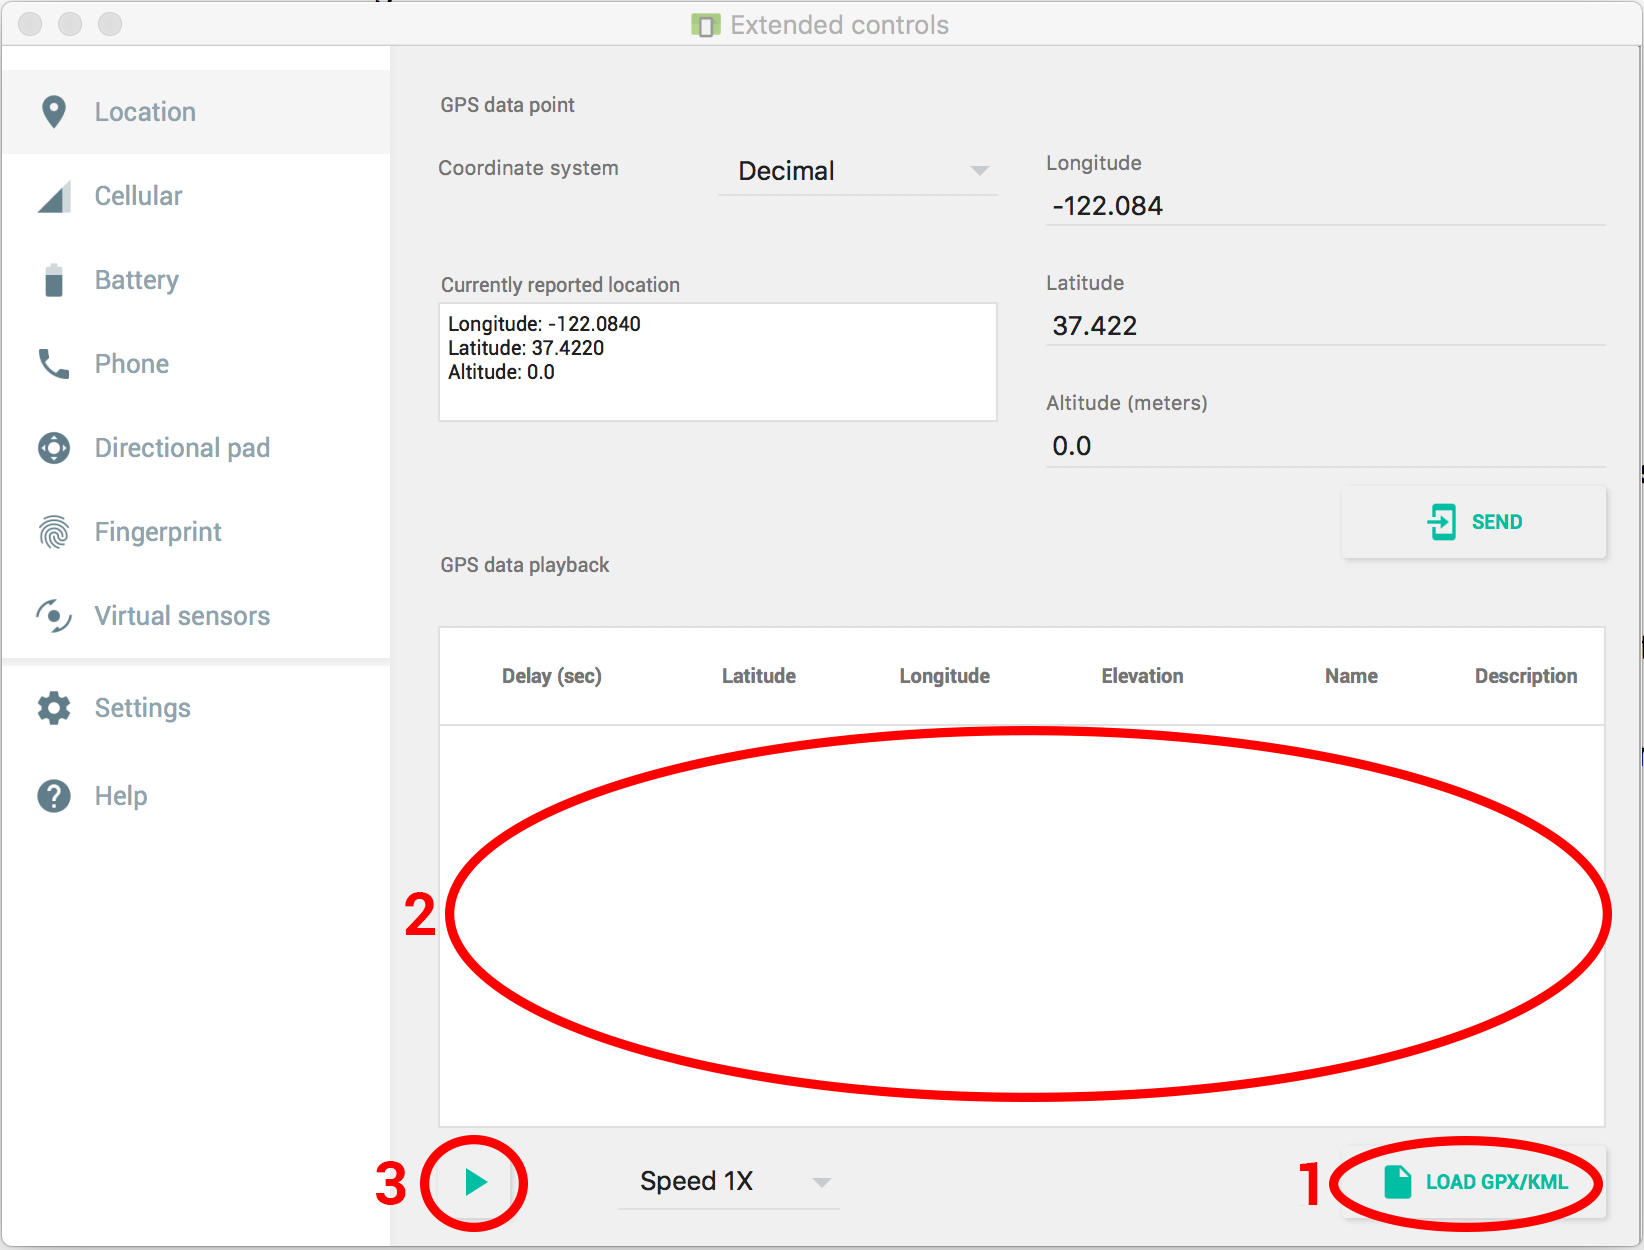
\includegraphics[width=\textwidth]{screenshots/EmulatorExtendedControls}
    \caption{Android Emulator Extended Controls}
    \label{fig:android-emulator-extended-controls}
  \end{minipage}
\end{figure}

\newpage
\subsection{Wegpunkt erreichen}

Sobald du den Wegpunkt erreicht hast, startet TravelBuddy deine Kamera.
Schiesse nun ein Foto der Sehenswürdigkeit. TravelBuddy überprüft anschliessend dein Foto,
stimmt dieses mit TravelBuddy überein, wird dir eine neue Route zum nächsten Punkt
angezeigt. Falls dein Foto nicht akzeptiert wird, nähere dich der Sehenswürdigtkeit und versuche es erneut.

\subparagraph{Hinweis Demoversion:}
Damit sich die Position auf der Karte verändert, können die zuvor geladenen GPS Punkte
abgespielt werden. Hierzu den ``Play'' Knopf im Dialog-Fenster
(\hyperref[fig:android-emulator-extended-controls]{Abbildung~\ref*{fig:android-emulator-extended-controls}}, Nr. 3) drücken.

Sobald ein Kamerabildschirm erscheint (\hyperref[fig:android-emulator-camera]{Abbildung~\ref*{fig:android-emulator-camera}}) den ``Stop'' Knopf im Dialog-Fenster
(\hyperref[fig:android-emulator-extended-controls]{Abbildung~\ref*{fig:android-emulator-extended-controls}}, Nr. 3) drücken.
Nachdem ein Foto erstellt und akzeptiert wurde, können die GPS Punkte wieder weiter abgespielt werden.

Die GPS Punkte sind so ausgelegt, dass zwischendurch ein falscher Weg eingeschlagen wird und
TravelBuddy einen neuen Weg errechnen muss.

\begin{figure}
  \centering
  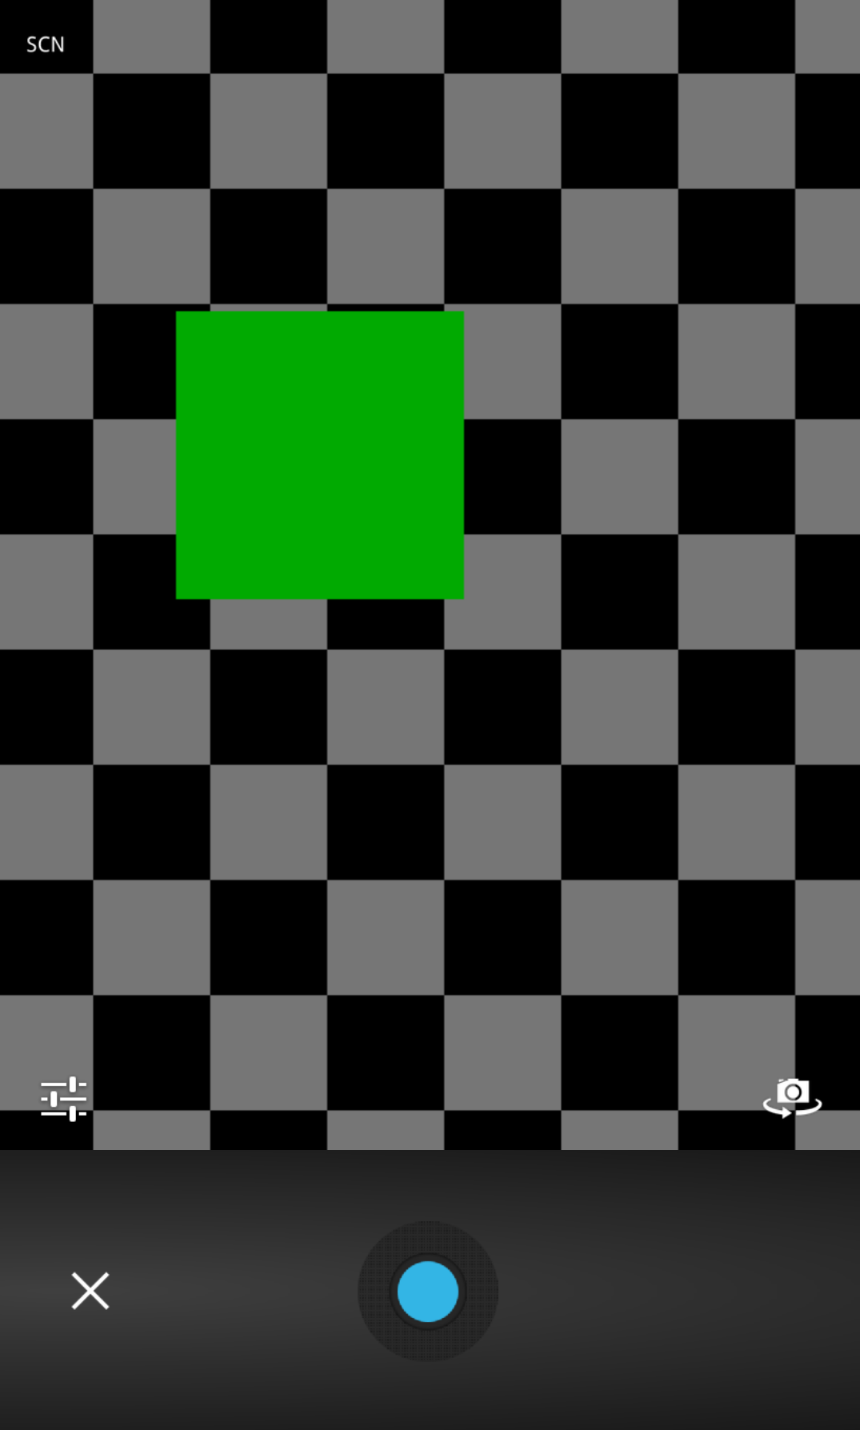
\includegraphics[width=0.48\textwidth]{screenshots/EmulatorCamera}
  \caption{Kamera Ansicht im Android Emulator}
  \label{fig:android-emulator-camera}
\end{figure}

\newpage
\subsection{Tour abschliessen}
Sobald du den letzten Wegpunkt deiner Tour erreicht hast, zeigt dir TravelBuddy eine
Übersicht über deine gesamte Tour an (\hyperref[fig:summary-activity]{Abbildung~\ref*{fig:summary-activity}}).

Sobald du auf ``Choose new tour'' tippst, gelangst du wieder auf den Startbildschirm von TravelBuddy.

\begin{figure}
  \centering
  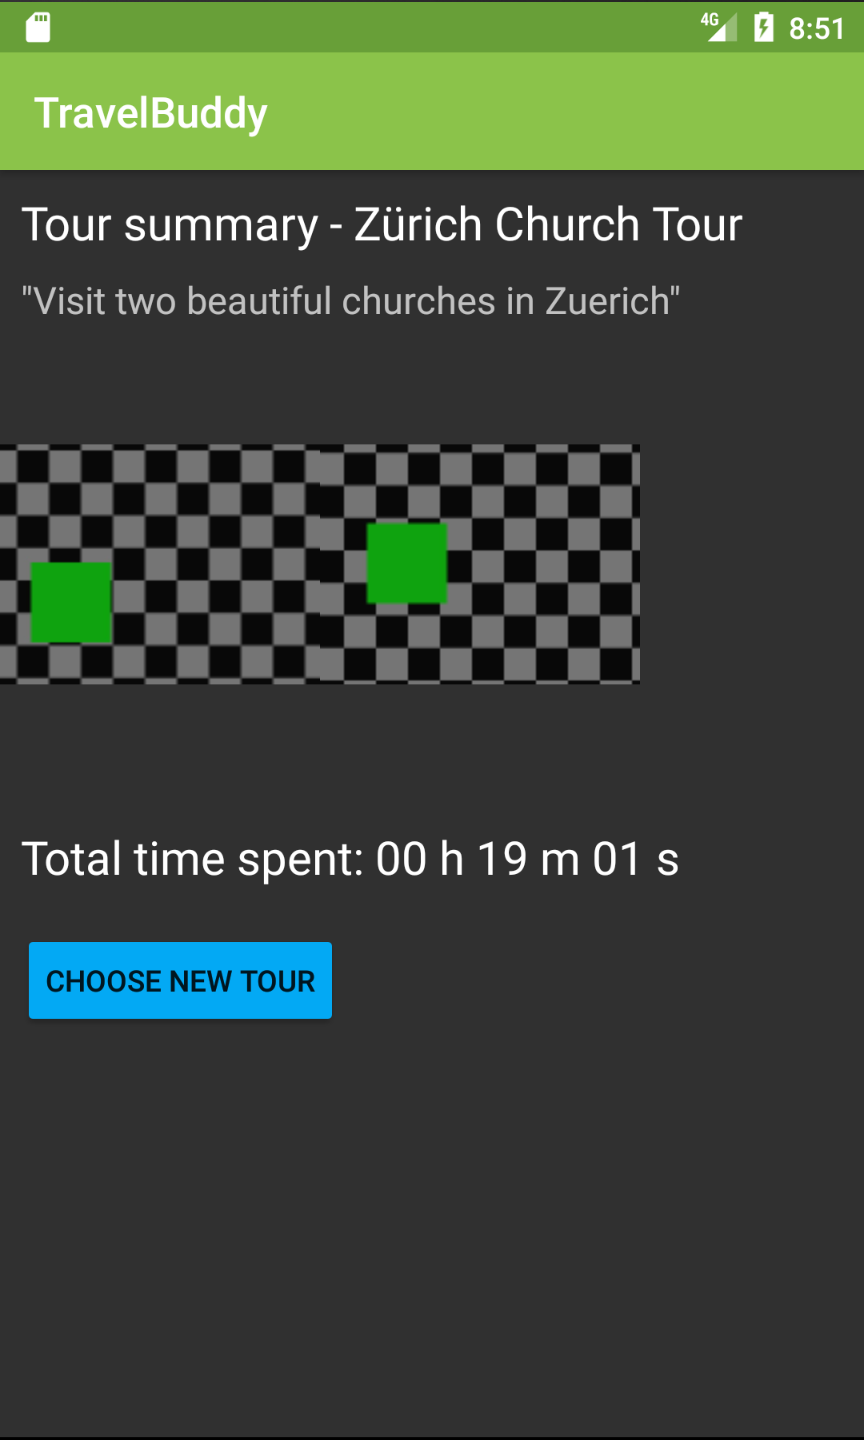
\includegraphics[width=0.48\textwidth]{screenshots/SummaryActivity}
  \caption{Übersicht über deine Tour}
  \label{fig:summary-activity}
\end{figure}
\end{document}
